% !TeX encoding   = UTF-8
\documentclass[12pt]{article}

\usepackage{sbc-template}

\usepackage{graphicx,url}
\usepackage[brazil]{babel}
\usepackage[utf8]{inputenc}
\usepackage{graphicx}	%Package para figuras
\usepackage{enumerate}
\usepackage{tabularx}
\usepackage{multirow}
\usepackage[linesnumbered,ruled,vlined]{algorithm2e}
\usepackage[table,xcdraw]{xcolor}
     
\sloppy

\title{Proposta do Trabalho Final PAA:\\ 
	   Encontrando os Top-K Influenciadores em uma Rede Social}

\author{Vagner Clementino\inst{1}}

\address{Departamento de Ciência da Computação\\
		Universidade Federal de Minas Gerais (UFMG)\\
 \email{vagnercs@dcc.ufmg.br}
}

\begin{document} 

\maketitle

%\begin{abstract}
%  This meta-paper describes the style to be used in articles and short papers
%  for SBC conferences. For papers in English, you should add just an abstract
%  while for the papers in Portuguese, we also ask for an abstract in
%  Portuguese (``resumo''). In both cases, abstracts should not have more than
%  10 lines and must be in the first page of the paper.
%\end{abstract}
     
%\begin{resumo} 
% To Do.
%\end{resumo}


\section{Introdução}
\label{sec:contexto}
Tradicionalmente as campanhas de marketing se baseiam em determinar um conjunto de consumidores, denominado público-alvo, e posteriormente focam suas ações naquela grupo \cite{hughes1996complete}{}. Neste contexto, a mineração de dados desempenha um papel fundamental por permitir a construção de modelos que tentam predizer o comportamento de um cliente baseado em seu histórico de compras \cite{kumar1999extracting}. Nos casos em que esta abordagem têm sucesso, foi possível perceber um aumento na lucratividade \cite{piatetsky1999estimating}. Contudo, este tipo de abordagem possui uma limitação básica: ela considera que a decisão de compra de uma pessoa é independente dos demais consumidores, desconsiderando o impacto que demais clientes, especialmente aqueles mais ``próximos", por ventura possam exercer.

O efeito que os demais consumidores possuem sobre a decisão de compra de um cliente é conhecido em Economia como \textit{externalidade da rede}{}. Com a expansão da Internet e do uso das redes sociais, este \textit{``efeito da rede"} têm se mostrado de suma importância em diversos setores, especialmente naqueles ligados diretamente à informação (software, imprensa, telecomunicações e etc.) \cite{shapiro2013information}{}.

Neste contexto, imagine que você trabalhe em uma empresa de marketing digital que pretende divulgar um novo produto \emph{A} da marca \emph{X} para o maior número possível de usuários em determinada rede social. Uma primeira estratégia seria divulgar o novo produto para cada usuário da rede, que é conhecida como marketing de massa. Tal opção é cara e baixa escalabilidade. Uma segunda alternativa seria apresentar o produto apenas ao usuários que \textit{seguem} a marca \textit{X}, utilizando, deste forma, um marketing direcionado. Esta estratégia peca pela sua abrangência, tendo em vista que não se tem a garantia que as informações do novo produto chegará aos demais usuários da rede social. Uma terceira via seria identificar um grupo de usuários tais que \textit{a partir deles é possível alcançar qualquer outro usuário da rede}{}. Ao escolher este grupo de usuários, também denominados \textit{``sementes"}, haverá uma maior probabilidade de que a informação chegue aos demais usuários. Este trabalho têm o foco nesta última abordagem.

A maneira que uma informação é propagada em uma rede é conhecida como \textit{Modelo de Propagação}. Neste sentido, a ``probabilidade" de propagação da informação dependerá naturalmente do modelo de difusão existente na rede. Contudo, neste trabalho,  parte-se da premissa que quanto maior o número de usuários que a informação pode alcançar maior será a propagação independente do modelo de propagação da rede. Na subseção \ref{subsec:problema_max_cobertura} iremos descrever o Modelo de Propagação adotado neste trabalho.

Uma rede social pode ser modelada como uma grafo não direcionado $G(V,E)${}, onde o conjunto de vértices $V$ representa os usuários e o conjunto de arestas $E$ representa os relacionamentos entre os mesmos. Na área de \textit{Teoria dos Grafos}, o problema de definir o conjunto $V^{'} \subseteq V${}, \textit{de tamanho mínimo}, tal que para todo vértice em $V^{'}$ é possível alcançar qualquer vértice em $V$ é conhecido como \textbf{Cobertura de Vértice}{}. A subseção \ref{subsec:problema_cobertura_vertice}{} define o problema formalmente.

Em um primeiro momento o conjunto $V^{'}$ (Cobertura de Vértice) poderia ser definida como as sementes da ação de marketing. Contudo, na prática, o tamanho de $V^{'}$ pode ser grande o suficiente de modo a inviabilizar o orçamento da campanha. Desta forma, se faz necessário encontrar um subconjunto de $W \subset V^{'}${} que alcance um maior número de pessoas sem, todavia, estourar o orçamento. Normalmente o tamanho deste subconjunto de $W^{'}$ deverá ser igual a $k$, onde $k$ é o número máximo de usuários que a campanha conseguirá patrocinar. O problema de encontrar $W$ tal que $|W| = k$ é conhecido na literatura como \textbf{Máxima Influência}{} e será definido formalmente na subseção \ref{subsec:problema_max_cobertura}{}.

\section{O Problema da Máxima Influência}
\label{sec:prob_max_influencia}

Seja $G=(V,E)$ um grafo não direcionado que modele uma rede social. A \textit{Máxima Influência} pode ser definido como o problema de encontrar u subconjunto $W \subset V^{'}${}, de modo que $\left\vert W \right\vert\leq K$ e $\cup_{j=1}^{k} w_{j}$ é \textit{maximizado}, onde $w_j \in V^{'}$ e $ 1 \leq j \leq k$.
Este pequeno conjunto de vértices têm a característica de que sua influência agregada na rede é maximizada.

O conceito de ``influência"{} é subjetivo e deve ser definido no contexto do problema estuado. Por exemplo, pode-se definir $w_{j} = 1$ caso o \textit{j-ésimo} usuário da rede foi influenciado na compra de um produto ou \textit{zero} caso contrário. Neste sentido, deve-se um buscar um conjunto mínimo de vértices que resulte em $\sum_{j=1}^{k} w_{j}$ \textit{máximo}. Neste trabalho, um vértice $u$ ``influencia" um outro $v$ se o fato de $u$ comprar um um produto faça com que $v$ também realize a mesma compra.

O processo de influenciação depende diretamente do \textit{Modelo de Propagação} utilizado para descrever a forma que vértices interagem na rede. Em síntese, um Modelo de Propagação define para cada vértice uma probabilidade de ativação e a influência é propagada por meio da ativação de vértices vizinhos por meio da probabilidade de ativação destes últimos. Este trabalho utiliza o modelo denominado \textit{Linear Threshold Model} \cite{granovetter1978threshold, schelling2006micromotives}{}, cujos detalhes são descritos na Subseção \ref{subsec:modelo_propagacao}.

Para modelo de propagação que foi considerado, o problema de determinar um valor de $k$ que maximize a influência é \textit{NP-Difícil} \cite{Garey:1979:CIG:578533,kempe2003maximizing}{}. Existe na literatura um algoritmo guloso que consegue um fator de aproximação da ordem de $1-\frac{1}{e}$ \cite{Hochbaum:1996:ACP:241938.241941}, onde $e$ é a base do logaritmo natural. Desta forma, no melhor caso existe uma garantia de desempenho um pouco acima de 63\%. O algoritmo guloso que consegue este é baseado na abordagem apresentada em \cite{domingos2001mining}. Assim qualquer trabalho  que proponha em resolver o problema da Máxima Influência pode considerar aquele valor como linha de base (``baseline"). Considerando que o Problema da Máxima Influência é \textit{NP-Difícil} se faz necessário a definição de uma heurística ou algoritmo aproximado a fim de o problema seja resolvido em situações reais. A Seção \ref{sec:heuristica} descreve a heurística proposta que é baseada na \textit{Cobertura de Vértice} \cite{Cormen:2009:IAT:1614191}{} de um grafo.

\section{Heurística Proposta}
\label{sec:heuristica}


A heurística proposta tem como objetivo determinar o conjunto $A_{0}$, também conhecido como sementes, tal que $A_{0} \in V$ e $|A_{0}| \leq k$ que maximize a influência em um grafo $G(V,E)${}. Considerando que a partir de um vértice $v \in V$ é possível alcançar um grande número de outros vértices, pode-se inferir que $v$ é um bom candidato para estar em $A_{0}$. Naturalmente os vértices pertencente à \textit{Cobertura de Vértices} do grafo que modela a rede social seriam a primeira alternativa.

\subsection{Heurística Baseada na Cobertura de Vértice}
\label{subsec:heuritica_vertex_cover}
O problema da \textit{Cobertura de Vértices} \cite{Garey:1979:CIG:578533}{} pode ser definido formalmente como segue: dado um grafo $G=(V,E)$ e um número inteiro $K\leq\left\vert V\right\vert$ verificar se existe uma cobertura de vértice de tamanho $K$ ou menos para $G$, isto é, se existe um subconjunto $V^{'} \subseteq V$ tal que $\left\vert V '\right\vert\leq K$ e, para cada vértice $\left\{ u,v\right\} \in E$, pelo menos um, $u$ ou $v$, pertence a $V^{'}${}. A figura \ref{fig_vertex_cover} ilustra um grafo com destaque para sua cobertura de vértice $V^{'}$ de tamanho 2.

\begin{figure}[!t]
\centering
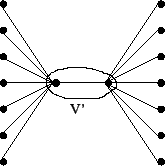
\includegraphics[width=2.0in]{../img/vertex_cover.png}
\label{fig_vertex_cover}
\caption{Cobertura de Vértice}
\end{figure}

Encontrar a Cobertura de Vértice mínima para um grafo $G=(V,E)$ qualquer é \textit{NP-completo}{} \cite{Garey:1979:CIG:578533, Cormen:2009:IAT:1614191}{}. Diante da inexistência de um algoritmo que retorna a solução exata em tempo polinomial, vem sendo propostos na literatura diversos \textit{algoritmos aproximativos}. Dentre eles, o mais utilizado, consegue executar em $O(V+E)$ em um nível de aproximação igual a \textit{2} \cite{Cormen:2009:IAT:1614191}, ou seja, seja $C^{*}$ uma cobertura de vértice ótima, o algoritmo retornará uma cobertura de vértice $C$, tal que $|C^{*}| \leq |C| \leq 2 \times |C^{*}|${}.

Na prática, caso utilizemos um algoritmo aproximativo de grau $2$, o tamanho da Cobertura de Vértice retornada será muito maior do que $k$. Neste sentido, se faz necessário encontrar dentro da Cobertura encontrada os $k$ vértices que maximizem a influência no grafo. Neste trabalho se realizou uma escolha gulosa dos vértices baseada na métrica denominada \textit{Degree Acesss}. O \textit{Degree Acesss} de um vértice $v$ de um grafo $G(V,E)$ é definido como total de vértices que são passíveis de serem alcançados a partir de $v$. O \textit{degree acesss} pode ser visto como o tamanho da contribuição exclusiva de um vértice para um possível cobertura de um grafo. A Figura mostra o valor do \textit{Degree Acesss} como ``label" de cada um dos vértices do grafo apresentado.

\begin{figure}[!t]
\centering
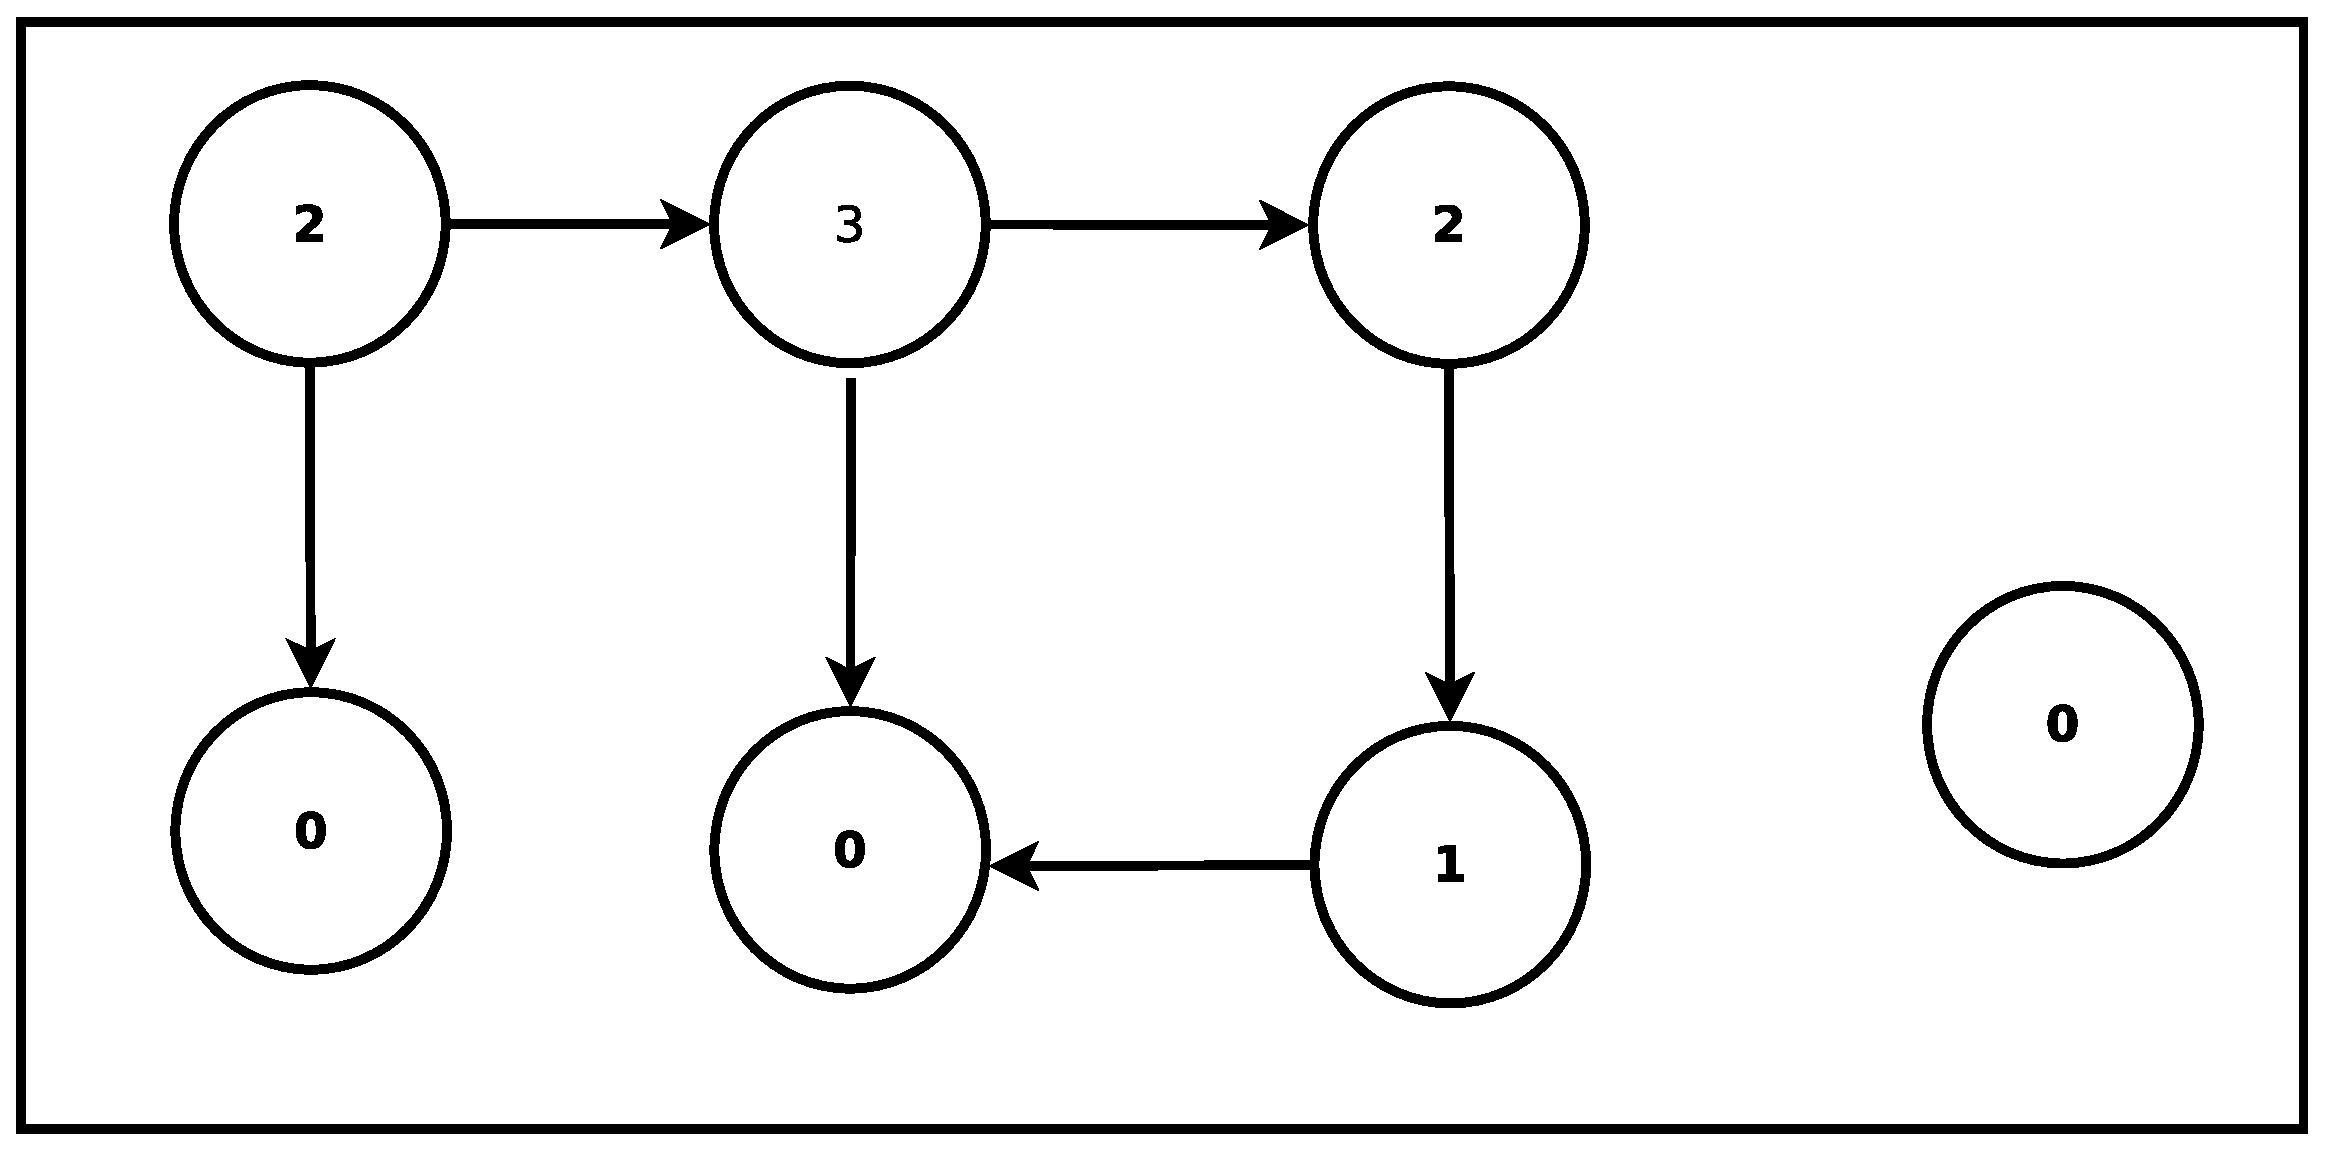
\includegraphics[width=4.5in]{../img/graph_deegree_acess.eps}
\label{fig_vertex_cover}
\caption{Degree Access para o vértice de um grafo}
\end{figure}


Com base na métrica proposta e na Cobertura de Vértice do grafo foi proposto a heurística descrita no Algoritmo \ref{algo:define_sementes} para determinar o conjunto $A_{0}$. Seja $C \in V$ a cobertura de vértice de um $G(V,E)$ obtida utilizando a heurística proposta em \cite{Cormen:2009:IAT:1614191}. O tamanho de $C$ é no máximo $ 2 \times C^{*}$, onde $C^{*}$ é a Cobertura de Vértice ótima para o grafo $G(V,E)$. Caso $|C| = k$ podemos naturalmente definir $A_{0} = C$. Do contrário, devemos encontrar em $C$ os $k$ vértices com o valor de \textit{degree acesss}{}.

\begin{algorithm}[!t]
\DontPrintSemicolon % Some LaTeX compilers require you to use \dontprintsemicolon instead
\SetKwFunction{FINVERTEXCOVER}{FIND-VERTEX-COVER}
\SetKwFunction{CALCULEDEGREEACESSS}{CALCULE-DEGREE-ACESSS}
\SetKwFunction{SORT}{SORT}
\SetKwFunction{DEQUEUE}{DEQUEUE}
\KwIn{Um grafo não direcionado e não ponderado $G(V,E)$\\
	  um inteiro $k$ correspondente a primeiro índice de $A$;\\
	  um inteiro $r$ correspondente ao último índice de $A$}
\KwOut{Um conjunto $A_{0} \in V$ tal que $ 1 \leq |A_{0}| \leq k$}
	
	$C \gets \emptyset$\;
	$A_{0} \gets \emptyset$\;
	$Q \gets \emptyset$ {$Q$ é uma fila}\;
	
	$C \gets $ \FINVERTEXCOVER{$G(V,E)$}\;
	\If{$|C| = k$}{
		
		$A_{0} \gets C$\;
		\Return{$A_{0}$}\;	
	
	}\Else{
	
		\CALCULEDEGREEACESSS{$G(V,E),C$}\;
		\SORT{$C$} {Ordenando o conjunto $C$ em ordem decrescente ao grau acessibilidade.}\;
		$Q \gets C${Atribuindo o conjunto $C$ para uma fila}\;
		\While{$|A| < k$ \textbf{or} $Q$ \textbf{is not} $\emptyset$} {
			
			$v \gets $ \DEQUEUE{$Q$}\;
			
			\If{$v.degreeAcess > 0$}{
			
				$A_{0} \gets A_{0} \cup v$\;
			
			}	
		}
		\Return{$A_{0}$}\;	
	}
\Return{$A_{0}$}\;
\caption{{\sc FIND-SEEDS} retorna o conjunto semente $A_0$ com base na Cobertura de Vértice de um grafo.}
\label{algo:define_sementes}
\end{algorithm}

Conforme pode ser observado o Algoritmo \ref{algo:define_sementes} utilizada uma estratégia gulosa, com base na Cobertura de Vértices, para definir o conjunto $A_{0}$. A Cobertura de Vértice é definida pelo método \textsc{FIND-VERTEX-COVER} que é baseado em \cite{Cormen:2009:IAT:1614191}{}. O calculo do \textit{degree acesss} é realizado pelo método \textsc{CALCULE-DEGREE-ACESSS}{}. Na subseção \ref{subsec:analise_complexidade} iremos analisar a complexidade de tempo e espaço do algoritmo como um todo.

Naturalmente, por se tratar de um heurística, a escolha gulosa proposta no Algoritmo \ref{algo:define_sementes} não resultará em uma solução ótima global. Todavia, espera-se que o conjunto $A_0$ definido desta forma resultará em um maior número de vértices ativos (conjunto $S$).

\subsection{Análise de Complexidade}
\label{subsec:analise_complexidade}

\subsubsection{Complexidade Temporal}
\label{subsubsec:complex_temporal}

A heurística descrita pelo Algoritmo \ref{algo:define_sementes} é baseada essencialmente nos métodos \textsc{FIND-VERTEX-COVER} e \textsc{CALCULE-DEGREE-ACESSS}{}. Conforme discutido anteriormente, o  \textsc{FIND-VERTEX-COVER} têm como base o um algoritmo aproximativo bastante conhecido \cite{Cormen:2009:IAT:1614191}{} cuja complexidade temporal é dada por $O(V+A)$.

O método \textsc{CALCULE-DEGREE-ACESSS}{} é baseado no conhecido algoritmo de busca em largura em grafos \textit{(Breadth-First Search - BFS)}. A ordem de complexidade temporal do BFS é dada por $O(V+A)$. Contudo, o método \textsc{CALCULE-DEGREE-ACESSS}{} é executado para vértice $c \in C$, onde $C$ é a Cobertura de Vértice. Como no pior caso $C = V$ temos que a contribuição de \textsc{CALCULE-DEGREE-ACESSS}{} na complexidade temporal é dada por $O(V^{2}+VA)${}. Como não há outro método com complexidade maior do que a do \textsc{CALCULE-DEGREE-ACESSS}{} podemos concluir que a \textit{complexidade temporal do Algoritmo \ref{algo:define_sementes}} é $O(V^{2}+VA)${}.

\subsubsection{Complexidade Espacial}
\label{subsubsec:complex_espacial}


A estrutura de dados básica utilizada neste trabalho foi um grafo a fim de representar uma rede social. A implementação neste trabalho utilizou um \textit{lista de adjacência} o que implica em uma complexidade espacial da ordem de $O(V+A)${}.


\section{Avaliação da Heurística}
\label{sec:avaliacao}

\subsection{Modelo de Propagação}
\label{subsec:modelo_propagacao}

Conforme exposto anteriormente, a fim de mensurar o valor $\cup_{j=1}^{k} w_{j}$ devemos definir um  \textit{Modelo de Propagação}. No trabalho proposto, será utilizado o modelo conhecido como \textit{Linear Threshold Model} \cite{granovetter1978threshold, schelling2006micromotives}{}. Neste modelo, um vértice $v$ é influenciado por cada um dos seus vizinhos $w$ de acordo com um peso $b_{v,w}$ que respeita a Equação \ref{eq:pesos_vizinhos}{}.

\begin{equation} \label{eq:pesos_vizinhos}
\sum\limits_{\textrm{w vizinho de v}}{b_{v,w} \leq 1}
\end{equation}

O problema da \textit{Máxima Influência} pode ser modelado como um grafo não direcionado $G(V,E)${}, onde o conjunto de vértices $V$ representa os possíveis consumidores e as arestas $E$ representam os relacionamentos entre os mesmos. O processo de propagação das informações utilizará \textit{Linear Threshold Model}. Desta forma, para cada consumidor $v \in V$ será atribuído aleatoriamente um threshold $\theta_v$ no intervalo $[0, 1]$. As arestas em $E$ serão ponderadas com os valores $b_{v,w}$ respeitando à Equação \ref{eq:pesos_vizinhos}. Cada vértice $v \in V$ terá um atributo determinando se ele está ativo, sendo que antes da execução do algoritmo todos estarão com o valor \textit{não ativo}{}.

Para cada vértice $v$ é definido aleatoriamente um \textit{threshold} $\theta_v$ no intervalo $[0, 1]$; este limiar representa a fração dos vizinhos que deve se tornar ativa para que o vértice $v$ torne-se ativo. Dada uma escolha aleatória dos \textit{threshold} e um conjunto inicial de nós ativos $A_{0}$ (sendo os demais nós inativos), o processo de difusão ocorre da seguinte forma: na etapa $t$, todos os nós que estavam ativos na etapa $t-1$ permanecem ativos, e um vértice $v$ qualquer se torna \textit{ativo} se o somatório dos pesos de seus vizinhos \textit{ativos} sejam $\geq \theta_v$, conforme Equação \ref{eq:ativacao}{}. Cabe ressaltar que o conceito de \textit{ativação} de um vértice depende do contexto que o modelo está sendo aplicado. Neste trabalho considera que um vértice $v$ foi ativado se ele comprou um determinado produto anunciado.

\begin{equation} \label{eq:ativacao}
\sum\limits_{\textrm{w é um vizinho ativo de v}}{b_{v,w} \geq \theta_v}
\end{equation}

Conforme pode ser observado, ao se aplicar \textit{Linear Threshold Model} o problema se resume em encontrar o conjunto $A_{0}$  tal que $|A_{0}| = k$ e que maximize o total de vértice ativos, denominado conjunto $S${}. É fácil verificar que $|S| = k$ antes da execução do algoritmo. 

\subsection{Análise Experimental}
\label{subsec:experimentos}

A fim de avaliar a heurística proposta se faz necessário  utilização de um conjunto de dados que apresente as características estruturais de uma rede social de grande escala. Desta forma, de maneira análoga ao trabalho de \cite{kempe2003maximizing}, foi utilizado um grafo de colaboração de coautorias em publicações de física \cite{snapnets}. Têm sido mostrado que redes de coautoria são capazes de capturar as principais características das redes sociais de modo mais geral \cite{newman2001structure}. Neste sentido, a utilização de uma rede coautoria possibilita resultados semelhantes àqueles obtidos de grafos de redes sociais.

O gráfico colaboração contém um vértice para cada pesquisador que tem pelo menos um artigo como coautor banco de dados da \textit{arXiv}\footnote{\url{http://arxiv.org/}}. Caso um artigo tenha dois ou mais autores, o dataset  possui uma aresta para cada par de autores. Observe que isso resulta em arestas paralelas quando dois pesquisadores estão como coautores de vários artigos. O gráfico resultante possui 9877 vértices e 51971 arestas e compreende de artigos publicados no período de janeiro de 1993 a abril de 2003 (124 meses). O data está disponível para download em \url{https://snap.stanford.edu/data/ca-HepTh.html}.

As baterias de teste consistirão da execução da heurística proposta por 10 (dez) vezes para diversos valores de $k$ 10 mil vezes. A cada nova execução os valores dos \textit{threshold} $\theta_v$ de cada vértice serão recalculados aleatoriamente com objetivo de remover qualquer viés que possa prejudicar os resultados do trabalho. Os dados que serão utilizados para comparação será o valor médio do conjunto $S$ obtido de todas as execuções. 

Visando comparar os resultados da heurística proposta com algum outro existente na literatura, foi escolhido o trabalho de \cite{kempe2003maximizing}. A opção por aquele trabalho se justifica pelo fato dele tentar resolver o mesmo problema utilizando, dentre outros o {Linear Threshold Model}{}. Para que a comparação pudesse ser realizada foi escolhido o mesmo \textit{dataset}\footnote{\url{https://snap.stanford.edu/data/ca-HepTh.html}} e os mesmos valores de $k$ escolhidos pelos autores.

Em \cite{kempe2003maximizing} é proposto um algoritmo guloso que adiciona vértices ao conjunto $A_{0}$ visando maximizar o conjunto de vértices ativados (conjunto $S$). Os autores não entraram em detalhes sobre como escolheram vértices que efetivamente aumentam o tamanho de $S$. Todavia, eles utilizaram três outras heurísticas para validar o seu trabalho:

\begin{itemize}
	\item Na primeira abordagem os vértices em $A_{0}$ forame escolhidas randomicamente;
	\item Na segunda heurística, foram escolhidos $k$ vértices em ordem decrescente de seus graus $d_{v}$;
	\item A terceira abordagem utilizou o conceito de \textit{Distance centrality} \cite{scott2012social}, que é uma  medida influência largamente utilizada na sociologia, e parte do pressuposto de que vértices mais próximos terão mais chances de influenciar uns aos outros.
\end{itemize}

A heurística proposta por \cite{kempe2003maximizing}	teve um desempenho satisfatório como o baseline por eles utilizados. A Figura \ref{fig:baseline} exibe os o total de vértices ativados para cada valor de $k$ para heurística proposto por Kempe et. al (linha "greedy") comparada com as demais heurísticas. Conforme exposto, o artigo citado não há a detalhes da implementação do algoritmo proposto, contudo, podemo será utilizados os resultados reportados para fim de comparação.

\begin{figure}[!t]
	\centering
	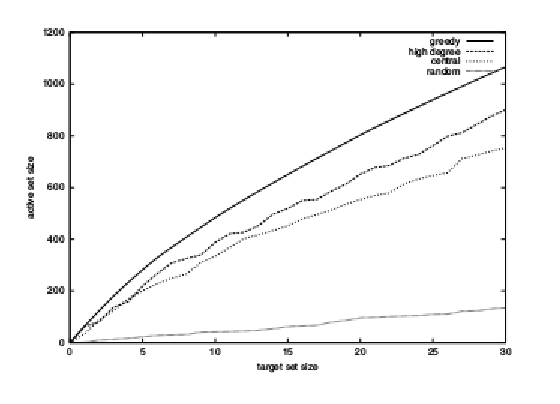
\includegraphics[width=5.0in]{../img/grafico_baseline.eps}
	\label{fig:baseline}
	
\end{figure}
 
Os testes foram executados em computador com o sistema operacional Ubuntu versão 12.04 kernel 3.13.0-37-generic 64 bits e com 4GB de memória RAM. A bateria de testes teve um tempo total de execução superior à 10 horas.

\section{Resultados}
\label{sec:resultados}

A Tabela \ref{tab:resultados} exibe os resultados das 10 (dez) execuções do algoritmo para alguns valores de $k$. A coluna ``Baseline"{} apresenta o total de vértices ativados no trabalho de \cite{kempe2003maximizing}{}. É possível verificar que os total de vértices ativados foi maior para todos os valores de k, tanto em média quanto na mediana. É possível verificar houve um baixo desvio padrão ($\sigma$) entre as dez execuções, exceção feita para $k=20$ em o total de vértices ativos no final da execução foi igual a $k$ (zero ativações adicionais) o que explica um maior desvio para aquela configuração.

\begin{table}[h]
\centering
\resizebox{\textwidth}{!}{%
\begin{tabular}{|c|c|c|c|c|c|c|c|c|}
\hline
\rowcolor[HTML]{C0C0C0} 
{\bf $|V|$} & {\bf $|C|$} & {\bf $\frac{|C|}{|V|}$} & {\bf $k$} & {\bf Média($\bar{x}$)} & {\bf Mediana ($\mu$) } & {\bf Devio Padrao($\sigma$)} & {\bf Valor Máximo} & {\bf Baseline} \\ \hline
 &  &  & 5 & 2153,8 & 2150,5 & 17,24 & 2193 & 200 \\ \cline{4-9} 
 &  &  & 10 & 2156,4 & 2153,5 & 20,33 & 2194 & 480 \\ \cline{4-9} 
 &  &  & 15 & 2160,6 & 2157,5 & 22,92 & 2199 & 600 \\ \cline{4-9} 
 &  &  & 20 & 1937,4 & 2153 & 674,43 & 2190 & 790 \\ \cline{4-9} 
 &  &  & 25 & 2208,4 & 2204,5 & 16,04 & 2238 & 950 \\ \cline{4-9} 
\multirow{-6}{*}{9877} & \multirow{-6}{*}{8434} & \multirow{-6}{*}{0,85} & 30 & 2162,3 & 2161,5 & 13,80 & 2184 & 990 \\ \hline
\end{tabular}
}
\caption{Resultados para diversos valores de k}
\label{tab:resultados}
\end{table}

A Figura \ref{fig:grafico_comparativo} exibe um comparativos dos resultados obtidos pela heurística (vide coluna Valor Máximo) com aqueles descritos em \cite{kempe2003maximizing}. É possível verificar que a heurística conseguiu valores melhores em todos os valore de $k$, tenho um valor bastante superior mesmo para valor de $k$ menores. Também é possível que a variação do total de vértices ativados não acompanha o mesmo crescimento de $k$. Esta tendência pode ser observado na Figura \ref{fig:grafico_comparativo} bem como por meio do valor do desvio padrão $\sigma$ da coluna Valor Máximo. O valor de $\sigma$ é dado por $19,41$ um valor relativamente baixo. Neste sentido, considerando os valores obtidos pela heurística um valor de $k= 25$ seria o ideal.

A tabela \ref{tab:ic_fracao} mostra a fração de vértices ativados para um intervalo de confiança igual a 95\% ($\lambda=0.05$){}\cite{jain2008art}. Conforme pode ser observado para a maiores dos valores de $k$ o percentual de vértices que ficariam ativados está na faixa de $21-22\%$. Este valor é obtido mesmo para valores pequenos de k ($k=5$), todavia, não altera como o crescimento do $k$ o que possivelmente é causado pela sobreposição influência entre os vértices.

% Please add the following required packages to your document preamble:
% \usepackage{graphicx}
% \usepackage[table,xcdraw]{xcolor}
% If you use beamer only pass "xcolor=table" option, i.e. \documentclass[xcolor=table]{beamer}
\begin{table}[h]
\centering
\resizebox{\textwidth}{!}{%
\begin{tabular}{|c|c|c|c|c|c|}
\hline
\rowcolor[HTML]{C0C0C0} 
{\bf k} & {\bf MEDIA($\bar{x}$)} & {\bf DESV PADRAO($\sigma$)} & {\bf IC} & {\bf MIN} & {\bf MAX} \\ \hline
5 & 0,21806 & 0,00175 & 0,00108 & 0,21698 & 0,21914 \\ \hline
10 & 0,21833 & 0,00206 & 0,00128 & 0,21705 & 0,21960 \\ \hline
15 & 0,21875 & 0,00232 & 0,00144 & 0,21731 & 0,22019 \\ \hline
20 & 0,19615 & 0,06828 & 0,04232 & 0,15383 & 0,23847 \\ \hline
25 & 0,22359 & 0,00162 & 0,00101 & 0,22258 & 0,22460 \\ \hline
30 & 0,21892 & 0,00140 & 0,00087 & 0,21806 & 0,21979 \\ \hline
\end{tabular}
}
\caption{Intervalo de confiança $\lambda = 0.05$ para a fração de vértices ativados}
\label{tab:ic_fracao}
\end{table}
Apesar dos resultados se mostrarem superiores aqueles obtido por \cite{kempe2003maximizing}, a heurística proposta ainda está bem abaixo do melhor algoritmo descrito na literatura para problema \cite{Hochbaum:1996:ACP:241938.241941} que consegue um total de vértices ativado da ordem de $63\%${}.	
		


\begin{figure}[ht]
	\centering
	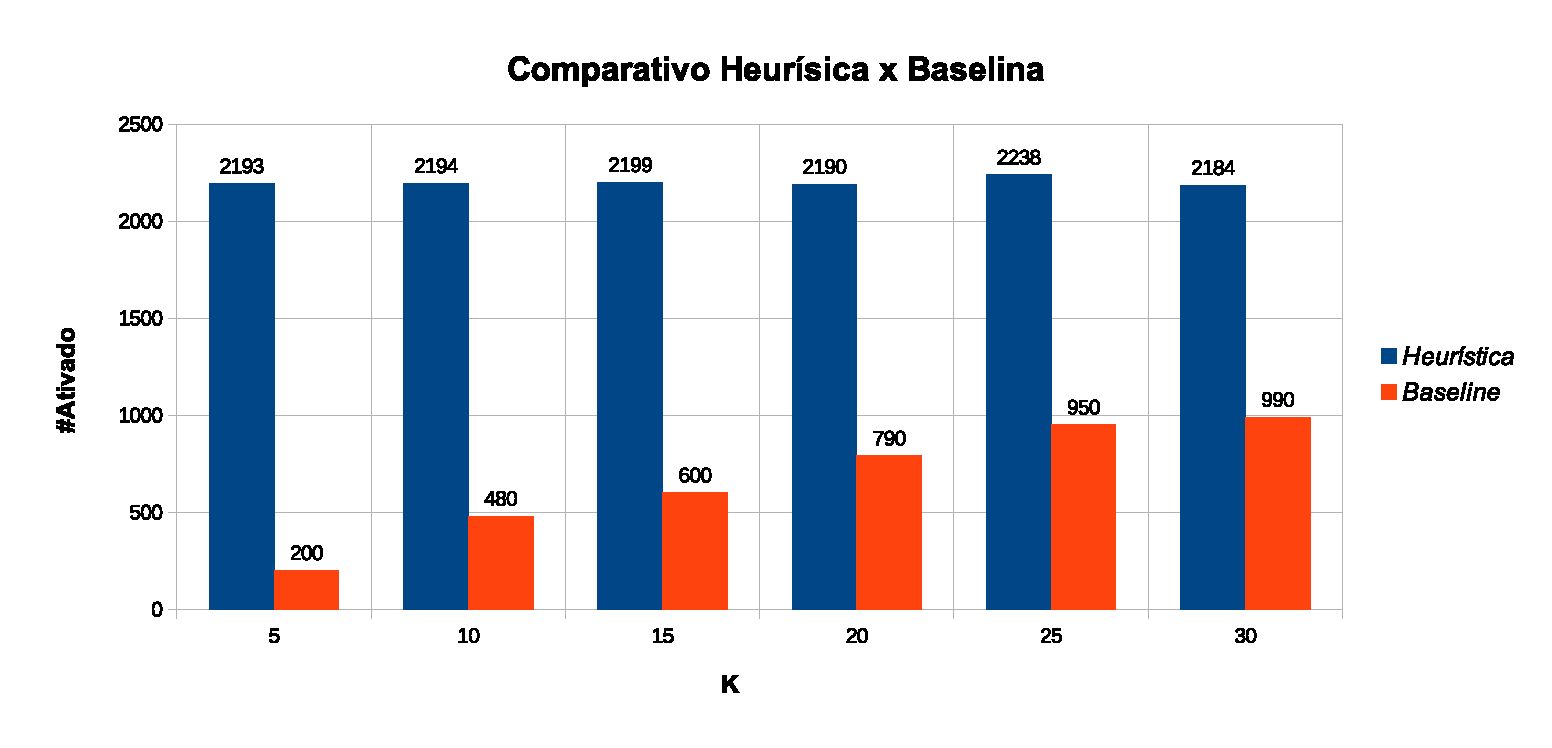
\includegraphics[width=6.5in]{../img/grafico_comparativo.eps}
	\label{fig:grafico_comparativo}
	\caption{Comparativo dos resultados da heurística com o do baseline}

\end{figure}

\section{Trabalhos Relacionados}
\label{sec:trab_relacionados}

No trabalho de \cite{domingos2001mining} é proposto um modelo com o objetivo de mensurar o valor da rede sobre um consumidor, ou seja, a receita esperada pelo fato de um consumidor influenciar a compra de um produto por outro usuário na rede. Os autores avaliam a abordagem proposta em um banco de dados de filtragem colaborativa. Este trabalho é um dos pioneiros com relação a avaliação do efeito na rede na probabilidade de compra de um consumidor. 

Em \cite{richardson2002mining} é realizada uma mineração de dados em redes sociais com o objetivo de construir um modelo probabilístico que possibilite melhor plano para um ``marketing viral"{}. Os resultados possibilitaram a redução do custo do marketing por consumidor, além do mais a abordagem é escalável o que mostra sua possível aplicação em dados de redes sociais reais.

No artigo \ref{chen2009efficient} é proposto uma heurística para resolver o Problema Máxima Influência. Os objetivos do trabalho são superar o algoritmo guloso original proposto por \cite{kempe2003maximizing} no tocante à reduzir o tempo de execução e propor novas heurísticas que visem melhorar a abrangência da influência dentre da rede. Os resultados mostraram uma melhoria de $15\%$ a $34\%$ no tempo de execução da abordagem proposta. 

Em \cite{kempe2003maximizing} é proposto um algoritmo guloso para solucionar o problema da Máxima Influência. Eles utilizaram três outras heurísticas visando avaliar o seu algoritmo: $(i)$ na primeira abordagem os vértices em $A_{0}$ forame escolhidas randomicamente; $(ii)$ na segunda heurística, foram escolhidos $k$ vértices em ordem decrescente de seus graus $d_{v}$; $(iii)$ A terceira abordagem utilizou o conceito de \textit{Distance centrality} \cite{scott2012social}, que é uma  medida influência largamente utilizada na sociologia, e parte do pressuposto de que vértices mais próximos terão mais chances de influenciar uns aos outros.

\section{Ameaças à Validade}
\label{sec:ameacas}
		
Apesar dos resultados satisfatórios discutidos na Seção \ref{sec:resultados} algumas ameaças à validade devem ser discutidas. A primeira delas é o fato do Modelo de Propagação ser bastante artificial. Em um caso real o simples fato de alguns amigos compraram um produto não levará efetivamente que um consumidor também o compre. Como os resultados são diretamente dependentes do modelo de propagação, os resultados podem ser devidos à simplicidade do modelo. Existem modelos mais complexos \cite{goldenberg2001talk,goldenberg2001using}{} que podem ser aplicados com o objetivo de avaliar o impacto nos resultados.

Um segundo ponto a ser discutido é com relação a métrica \textsc{DEGREE ACESSS}{}. Não existe na literatura estudo que avaliem a efetividade da métrica na escolha de vértice que melhorem a influência na rede. Desta forma, um maior número de estudos deveriam ser realizados a fim de avaliar a métrica proposta. 

Para finalizar cabe ressaltar que a heurística foi aplicada em único grafo. Neste sentido, não há como generalizar os resultados. Desta forma, é primordial que o modelo ora proposto seja aplicado em diversos grafos que representem redes sociais como objetivo de verificar se a heurística é dependente ou não da estrutura da rede.

\section{Conclusões e Trabalhos Futuros}

Este trabalho se propôs em resolver o problema da Máxima Influência em uma rede social. A partir de uma heurística baseada na Cobertura de Vértice foi verificado o total de vértice que comprariam um determinado produto se um $k$ inicialmente realizassem a mesma compra. A propagação da influência foi realizada utilizando o modelo de propagação conhecido como \textit{Linear Threshold Model}{}. Foi proposto um algoritmo guloso que utiliza a métrica denominada \textsc{DEGREE ACESSS}{}.

A heurística proposta alcançou resultados satisfatórios em comparação com o baseline utilizado. Ademais, o modelo proposto é bem flexível o que possibilita refinamentos na métrica proposta. Como trabalhos futuros é proposto a aplicação da heurística em grafos reais para verificar a escalabilidade da mesma. Um outro desdobramento do trabalho é a utilização de outros característica das redes sociais em conjunto com o textsc{DEGREE ACESSS}{} para melhorar a escolha gulosa.			

\bibliographystyle{sbc}
\bibliography{../bib/proposta-ref}

\end{document}
